\clearpage
\section{ Problem 3.}
In $\mathbb{R}^2$, the weighted inner product is given by
$$ \langle x, y \rangle = ax_1y_1 + bx_2y_2 $$
where $a$ and $b$ are positive. Find a weighted inner product such that
the graph represents a unit circle as
\begin{figure}[H]
    \centering
    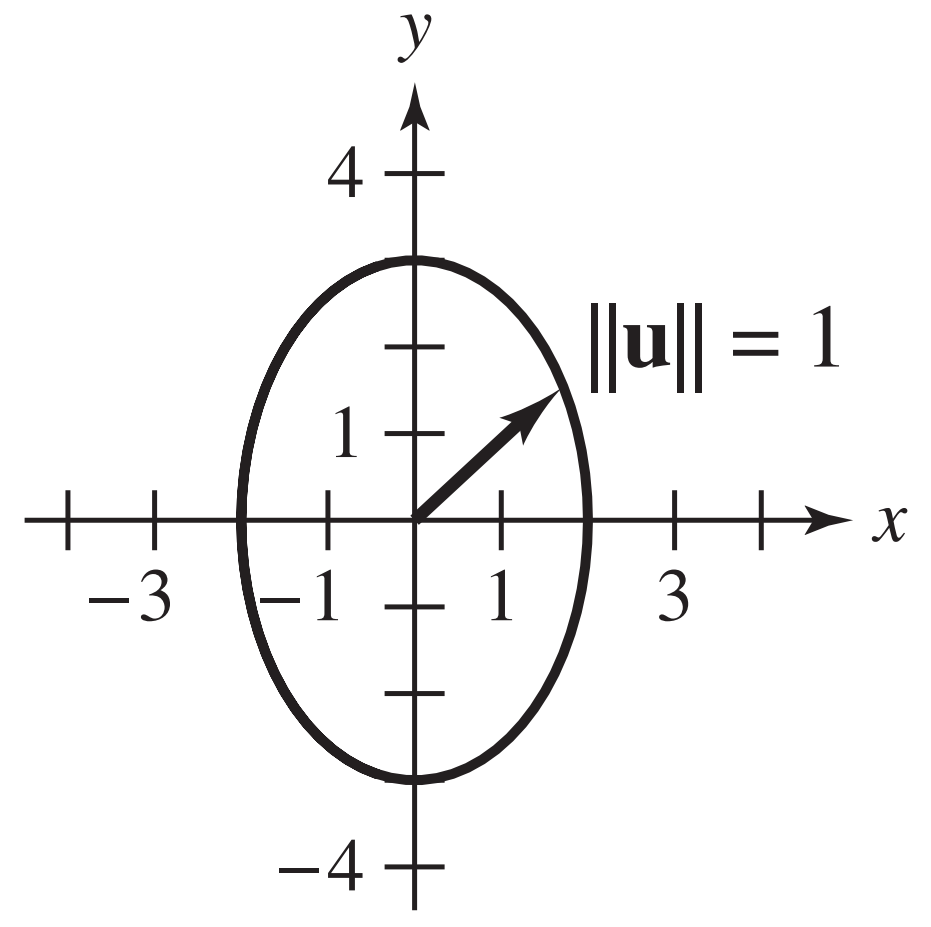
\includegraphics[width=6cm]{graphics/3_0.png}
    % \caption{}
\end{figure}
In that inner product space, reflect that unit circle about an input
plane.

\vspace*{1cm}

\textbf{Theory:}\\[6pt]
An inner product is a generalization of the dot product. In a vector space, it is a way to multiply vectors together, with the result of this multiplication being a scalar.\\[6pt]
Weighted inner products have exactly the same algebraic properties
as the “ordinary” inner product. But they introduce weights or importance factors that modify the calculations and geometric interpretations. \\[6pt]

The inner product is a fundamental concept that enables us to quantify the angle between vectors and establish measures of length, distance, orthogonality, and projections. \\[6pt]

In order to solve this problem, we need to first find the weighted inner product such that the graph represents a unit circle. Then, we need to reflect that unit circle about an input plane.\\[6pt]

\vspace*{1cm}

\textbf{Python code:}
\lstinputlisting[language=Python]{code/problem3.py}

\clearpage

\textbf{Result:}
\begin{figure}[H]
    \centering
    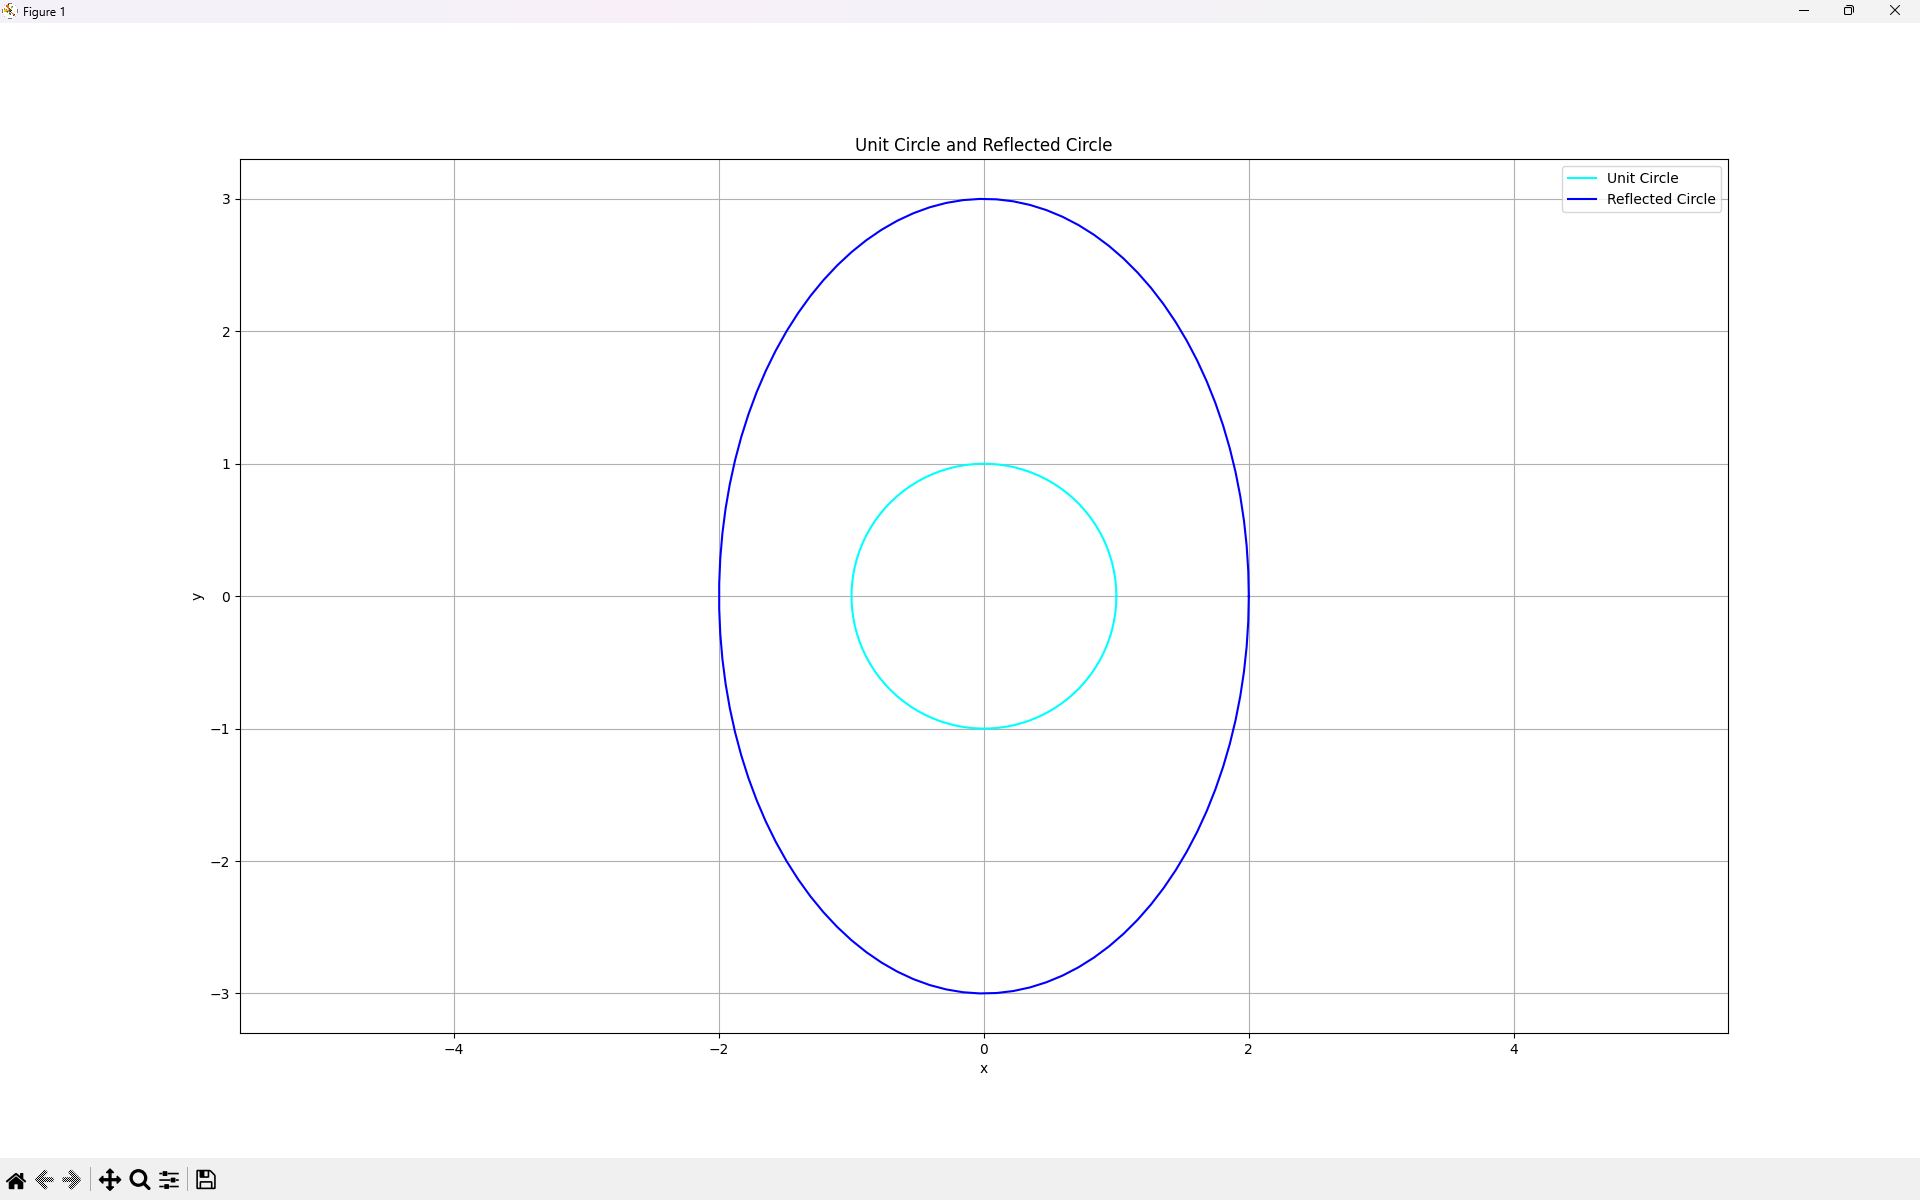
\includegraphics[width=16cm]{graphics/3.png}
    \caption{Console output of problem3.py}
\end{figure}